% Section content template for individual Educative lessons
% This file contains the actual content for a specific section
% Generated from Educative API section content

% Section: Introduction to SOLID Design Principles
% Section ID: 6732554378149888
% Section Slug: introduction-to-solid-design-principles
% Generated: 2025-12-11T05:49:40.716002

\subsection{Introduction}\label{introduction}
\\
When creating software, we can follow good practices to avoid issues to make our code easier to understand, robust, and maintainable. Few of these practices are often termed as principles, e.g., the \textbf{SOLID} principles refer to the best practices to be followed in OOD.
\\
SOLID is an acronym for the first five object-oriented design (OOD) principles by \emph{Robert C. Martin }, also known as \emph{Uncle Bob}, the author of \emph{Clean Code: A Handbook of Agile Software Craftsmanship.}
\\
The illustration below represents the acronym for SOLID design principles.

\begin{figure}[htbp]
 \centering
 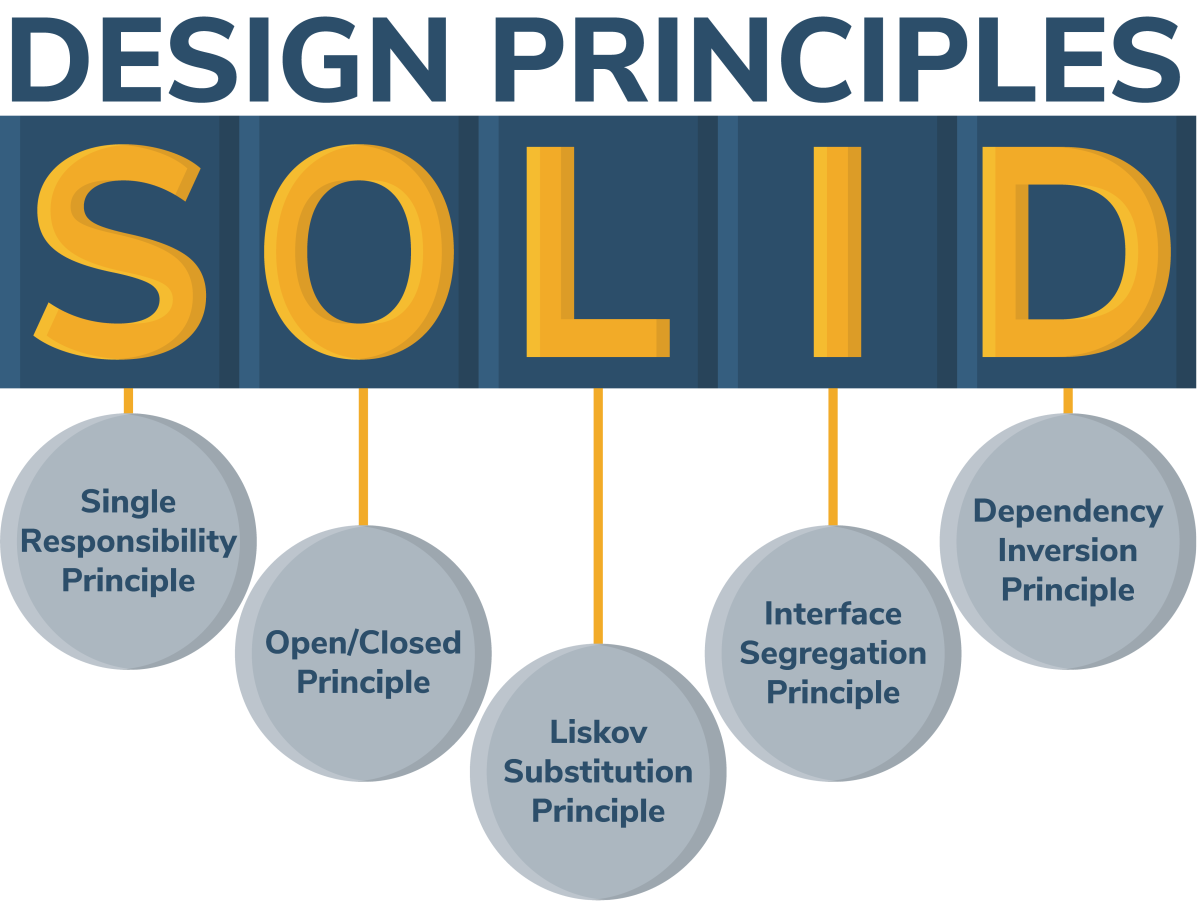
\includegraphics[width=0.35\textwidth]{Images/chapter_4/section_6732554378149888/5522800233414656.png}
 \caption{The SOLID design principle in object-oriented design}
\end{figure}

\subsection{Why use SOLID principles?}\label{why-use-solid-principles}
\\
Let's look at the possible issues below that may occur in the code if we don't adhere to the SOLID principles.

\begin{itemize}
\item
The code may become tightly coupled with several components, which makes it difficult to integrate new features or bug fixes and sometimes leads to unidentified problems.
\item
The code will be untestable, which effectively means that every change will need end-to-end testing.
\item
The code may have a lot of duplication.
\item
Fixing one issue results in additional errors.
\end{itemize}
\\
However, if we adhere to the SOLID principles, we are able to do the following:

\begin{itemize}
\item
Reduce the tight coupling of the code, which reduces errors.
\item
Reduce the code's complexity for future use.
\item
Produce more extensible, maintainable, and understandable software code.
\item
Produce the code that is modular, feature specific, and is extremely testable.
\end{itemize}

\subsection{Design principles}\label{design-principles}
\\
Let's look at the definition of the five design principles.

\begin{itemize}
\item
In the \textbf{Single Responsibility Principle (SRP)}, each class should be responsible for a single part or functionality of the system.
\item
In the \textbf{Open Closed principle (OCP)}, software components should be open for extension but closed for modification.
\item
In the \textbf{Liskov Substitution Principle (LSP)}, objects of a superclass should be replaceable with objects of its subclasses without breaking the system.
\item
The \textbf{Interface Segregation Principle (ISP)} makes fine-grained interfaces that are client specific.
\item
The \textbf{Dependency Inversion Principle (DIP)}, ensures that the high-level modules are not dependent on low-level modules. In other words, one should depend upon abstraction and not concretion.
\end{itemize}
\\
In the next few lessons, we will explain these five design principles in detail.

% End of section content